% Network I
\chapter{Network I}

% Tumour derived
\section{Tumour derived network} \label{s:ap:tum_net}

\Cref{fig:N_I:tum_leiden_modifiers} complements the work done in \cref{s:N_I:tum_describe} which explores the mutation burden across the genes used to construct the network.

\begin{figure}[H]    
    \centering
    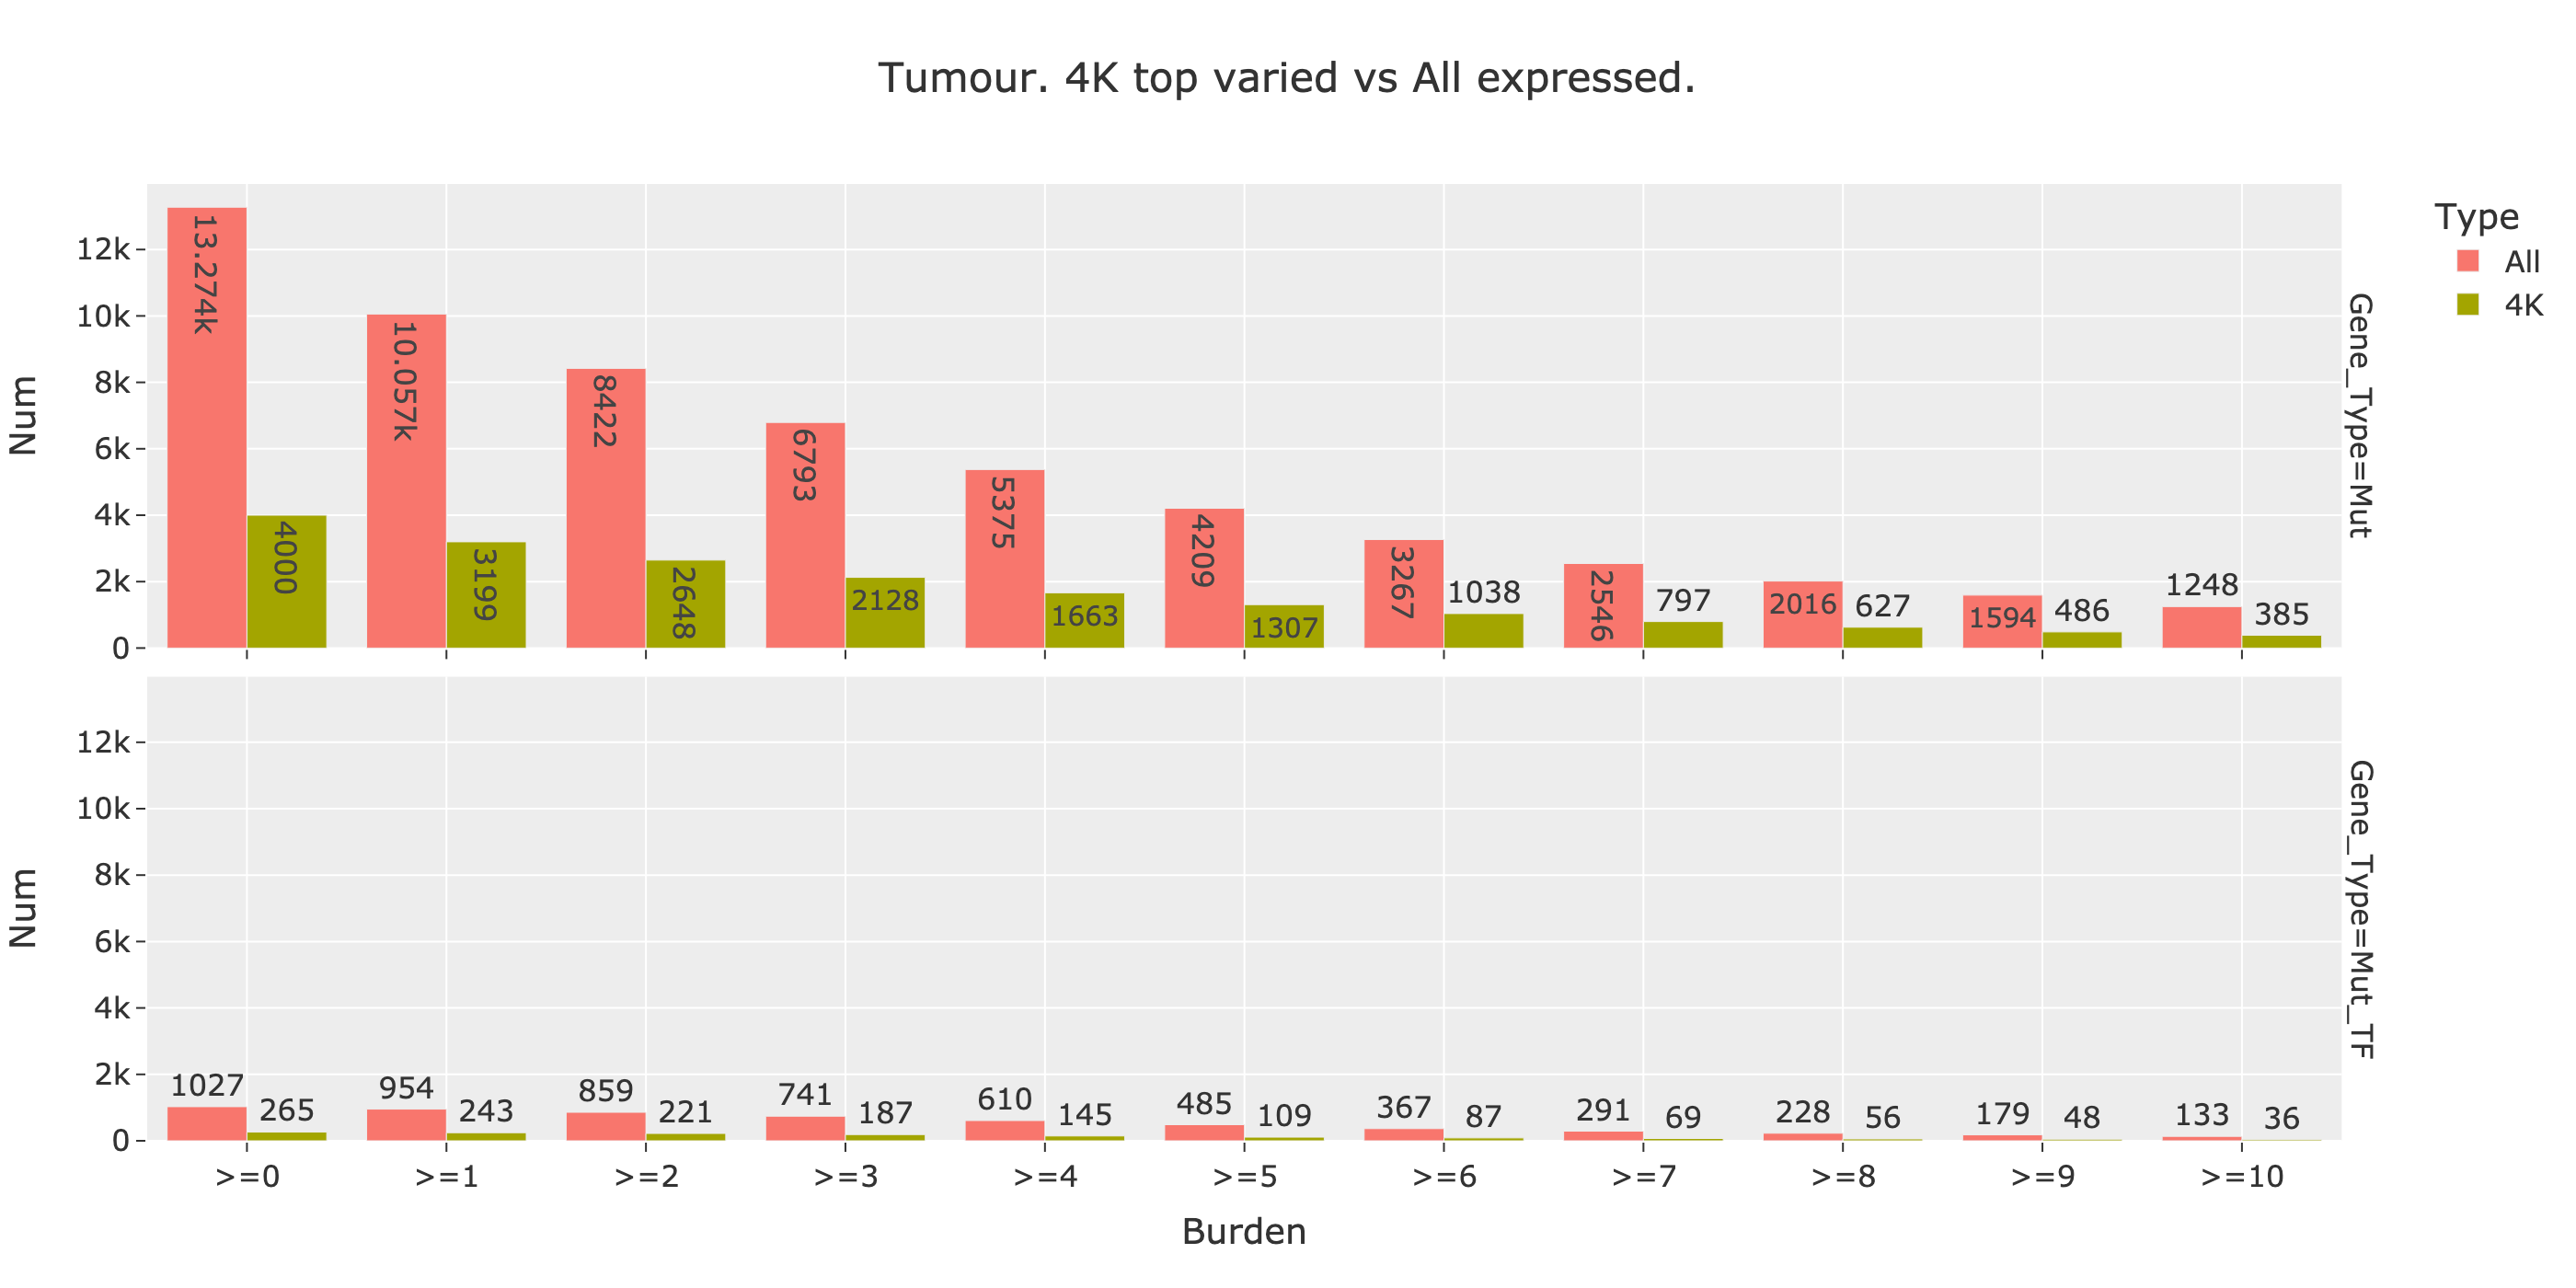
\includegraphics[width=1.0\textwidth,keepaspectratio]{Sections/Network_I/Resources/Tum_network/MutTF_representation_4K-all.png}
    \caption{How many genes are mutated in the 4K most varied genes compared to all the expressed genes. First plot includes all the genes TF and non-TF, while the bottom only the TFs. Overall the figure shows that there are a few genes with a high mutation burden included in the 4000 genes used to build the networks.}
    \label{fig:N_I:mut_rep_tum}
\end{figure}


% P0 derived network
\section{P0 derived network} \label{s:ap:P0}

% Clustering configuration
\subsection{Clustering analysis} \label{s:ap:P0_cs_analysis}

% Clustering model

% Explain what and why are the clustering methods we used
This work builds on the analysis of the P0 networks from \cref{s:p0}, using the first iteration of the network pipeline shown in \cref{fig:N_I:network_pipeline}. In this section, the cluster analysis steps developed in \cref{s:clustering_analysis} are applied to the MEV scores computed in the final stage of the network pipeline.

The clustering process involves running \acrfull{pca} and K-means to stratify MIBC based on gene expression. Based on the evaluation of three different clustering metrics (Silhouette, Calinski-Harabasz, and Davies-Bouldin), the following clustering models were selected\footnote{Other clustering methods explored included DBSCAN, MeanShift, Affinity Propagation, OPTICS, HDBSCAN, and Fuzzy K-means. The models retained are those that produced reasonable results, i.e., did not cluster the samples into only 1 or 2 clusters}. All models used the Scikit-learn implementation \cite{Scikit-learn_undated-ax}, including K-means, Agglomerative Clustering with Average linkage (Agg\_Avg), Ward, Gaussian Mixture Model, and Spectral Clustering.

\begin{figure}[!htb]
    \centering
    \begin{subfigure}[!t]{0.8\textwidth}
        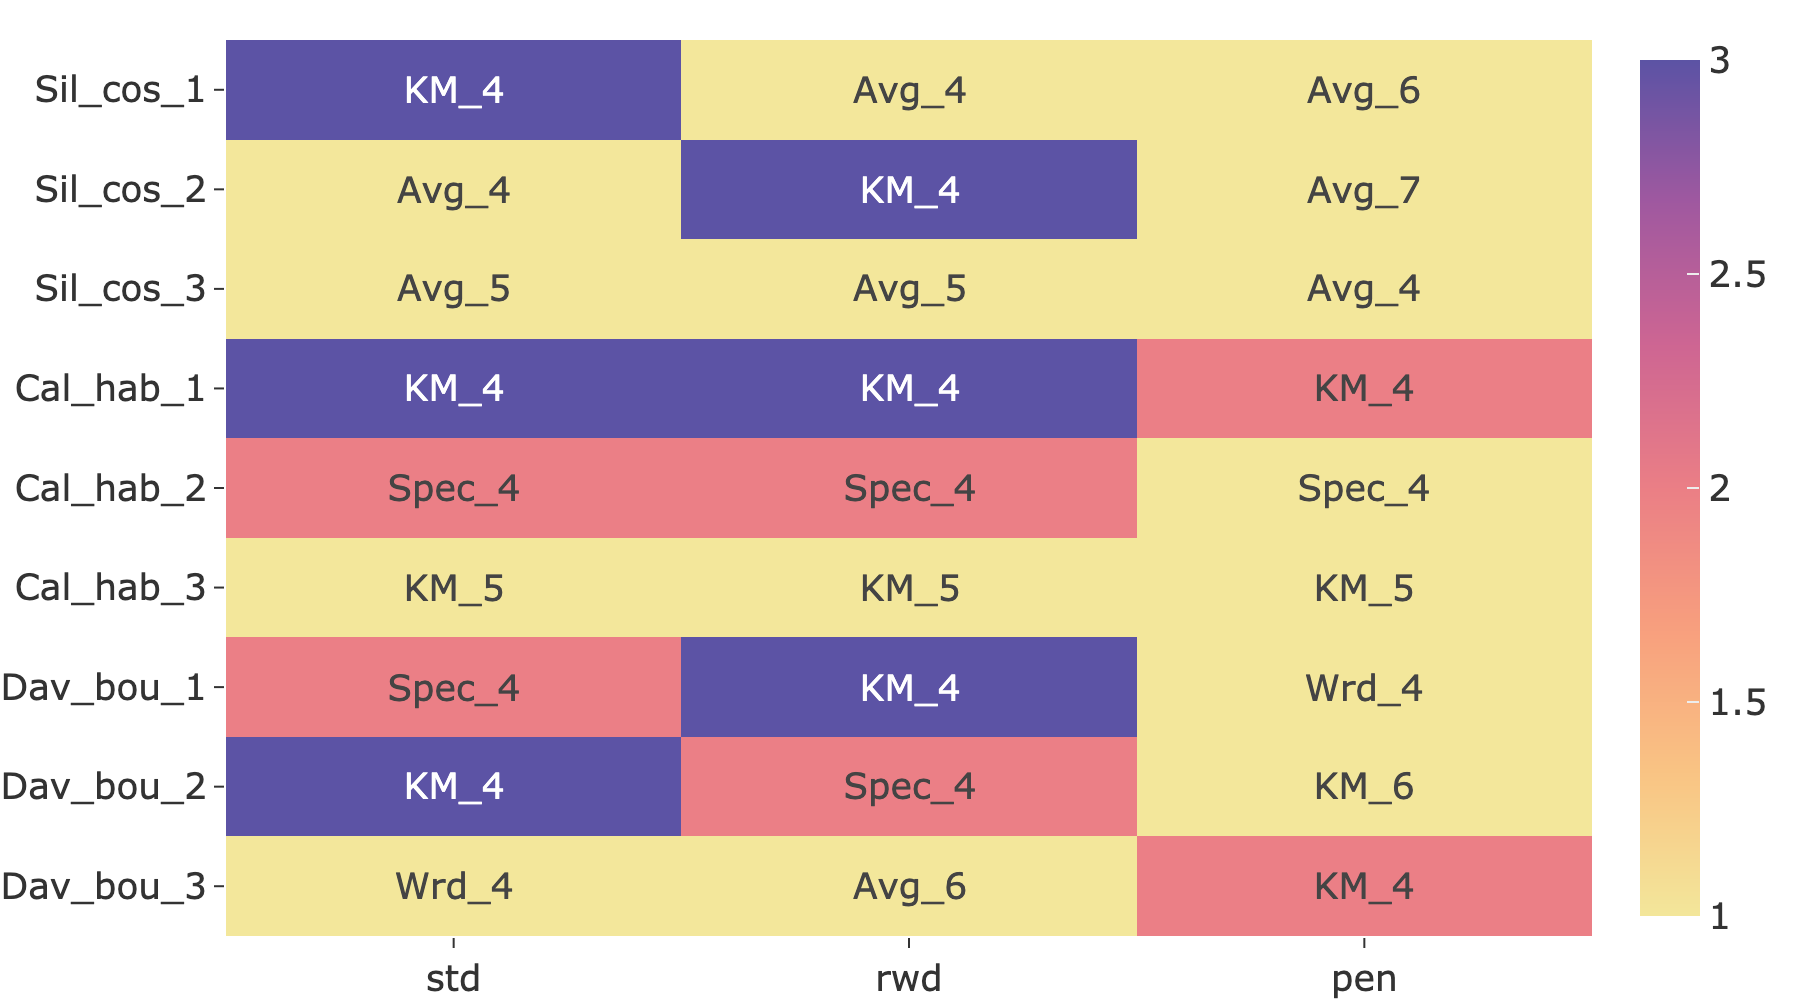
\includegraphics[width=\textwidth,keepaspectratio]{Sections/Network_I/Resources/P0/clustering/top3_cs_gen_p0_tum4K_50TF_v3.png}    
        \caption{Cluster model and size}
        \label{fig:N_I:p0_metr_model_size}
    \end{subfigure}
    \begin{subfigure}[!t]{0.8\textwidth}
        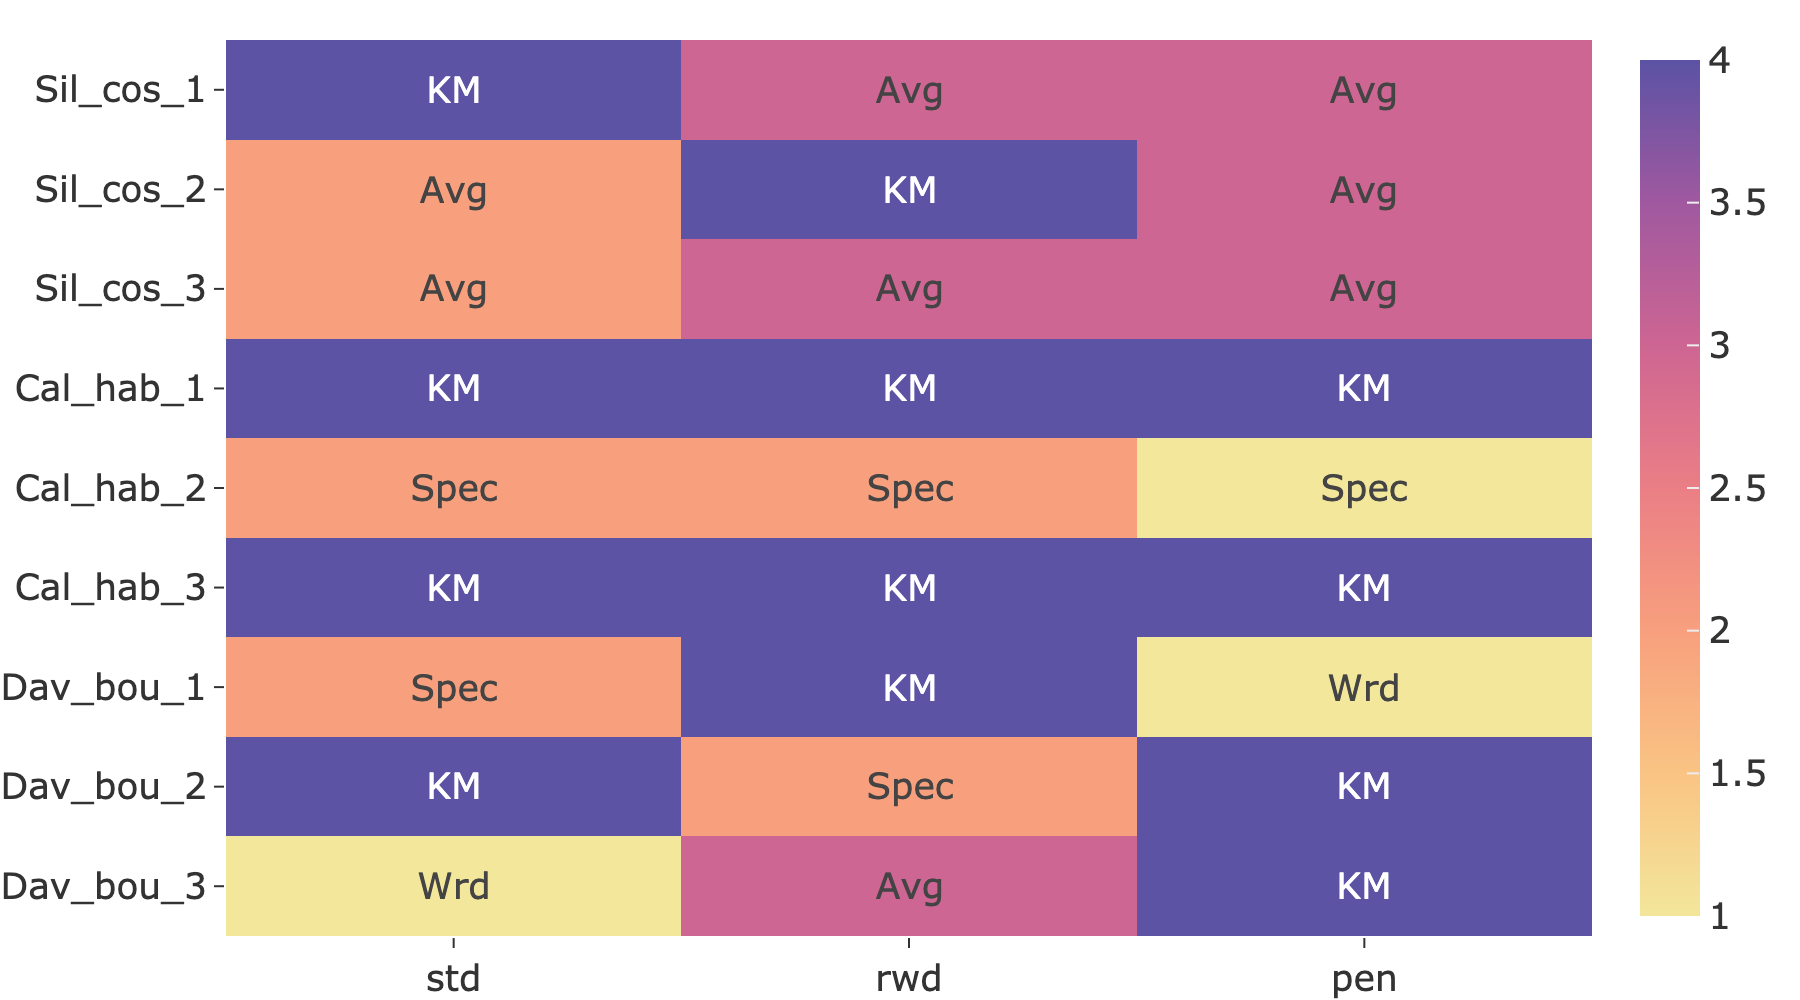
\includegraphics[width=\textwidth,keepaspectratio]{Sections/Network_I/Resources/P0/clustering/top3_cs_model_p0_tum4K_50TF_v3.png}
        \caption{Cluster model}
        \label{fig:N_I:p0_metr_model}
    \end{subfigure} 
    \caption{Clustering models for each network type with the top three clustering scores. Colouring scale corresponds to the encounter frequency \textbf{per network type}; i.e. the count restarts for every network. A) looks at the overall most common clustering model configuration. B) at the most common clustering model. The two heatmaps show that K-means with K=4 is the overall most performing clustering model. Agglomerative Clustering with average linkage and Spectral Clustering are the following candidates.}
    \label{fig:N_I:p0_top_3_metrics_I}
\end{figure}

% Introduce the results and motivate the reason why we don't include K=2,3
% Why not using the silhouette distribution
The clustering methods were applied to the MEV scores derived from the three networks (standard, reward, and penalised) with cluster sizes (K) ranging from 3 to 9, and the same clustering metrics were used to assess performance\footnote{Models with 2 or 3 clusters were not considered, as the metrics tend to give higher scores for models with 2 or 3 clusters}. Initially, the distributions of the three clustering metrics across the three P0-derived networks were used to inform the choice of clustering configuration, as was done in the analysis presented in the first chapter \cref{s:cs:right_config} - \cref{fig:cs:cs_metrics}. However, this approach proved challenging to present in this thesis and to isolate the prevailing trends for selecting the optimal clustering configuration across all three networks. Instead, using heatmaps of the top 3 best-performing clustering models was found to be more suitable for making global decisions, as shown in \cref{fig:N_I:p0_top_3_metrics_I,fig:N_I:p0_top_3_metrics_II}.

% Choosing the clustering model
\subsubsection*{Choosing the clustering model} \label{s:ap:p0_clustering}

Throughout the clustering configuration, K-means with K=4 consistently emerges as the top-performing clustering model across the subtypes from the three networks, as shown in \cref{fig:N_I:p0_metr_model_size}. This is followed by Spectral Clustering with K=4. In the heatmap displaying the frequency of the models, K-means consistently appears as the top-performing model, ranking in the top 3 of the clustering metrics across all networks 4 times. This is followed by Agglomerative Clustering, which appears 3 times in the top 3 within the reward and penalised networks; see \cref{fig:N_I:p0_metr_model}. The prevailing number of clusters, regardless of the clustering model, is K=4 across all MIBC subtyping derived from all networks, as indicated in \cref{fig:N_I:p0_metr_size}. This finding is further supported by the elbow method heuristic in \cref{fig:N_I:p0_elbow_method}.

% Narrowing down to the 2 clustering models
The clustering scores and analysis suggest that K-means with K=4 is the best-performing clustering model, as supported by all three metrics, and it is consistent across all three networks. This outcome differs from expectations based on earlier work in \cref{s:clustering_analysis}, where at least five clusters were identified using computational methods, with K=6 being informed by biological knowledge (IFNg groups). Additionally, K=4 is the next logical choice, as K=2 and K=3 were not considered due to their tendency to always exhibit the best K. Consequently, further analysis will focus on comparing the MIBC subtypes directly.


\begin{figure}[!t]
    \centering
    \begin{subfigure}[!t]{0.8\textwidth}
        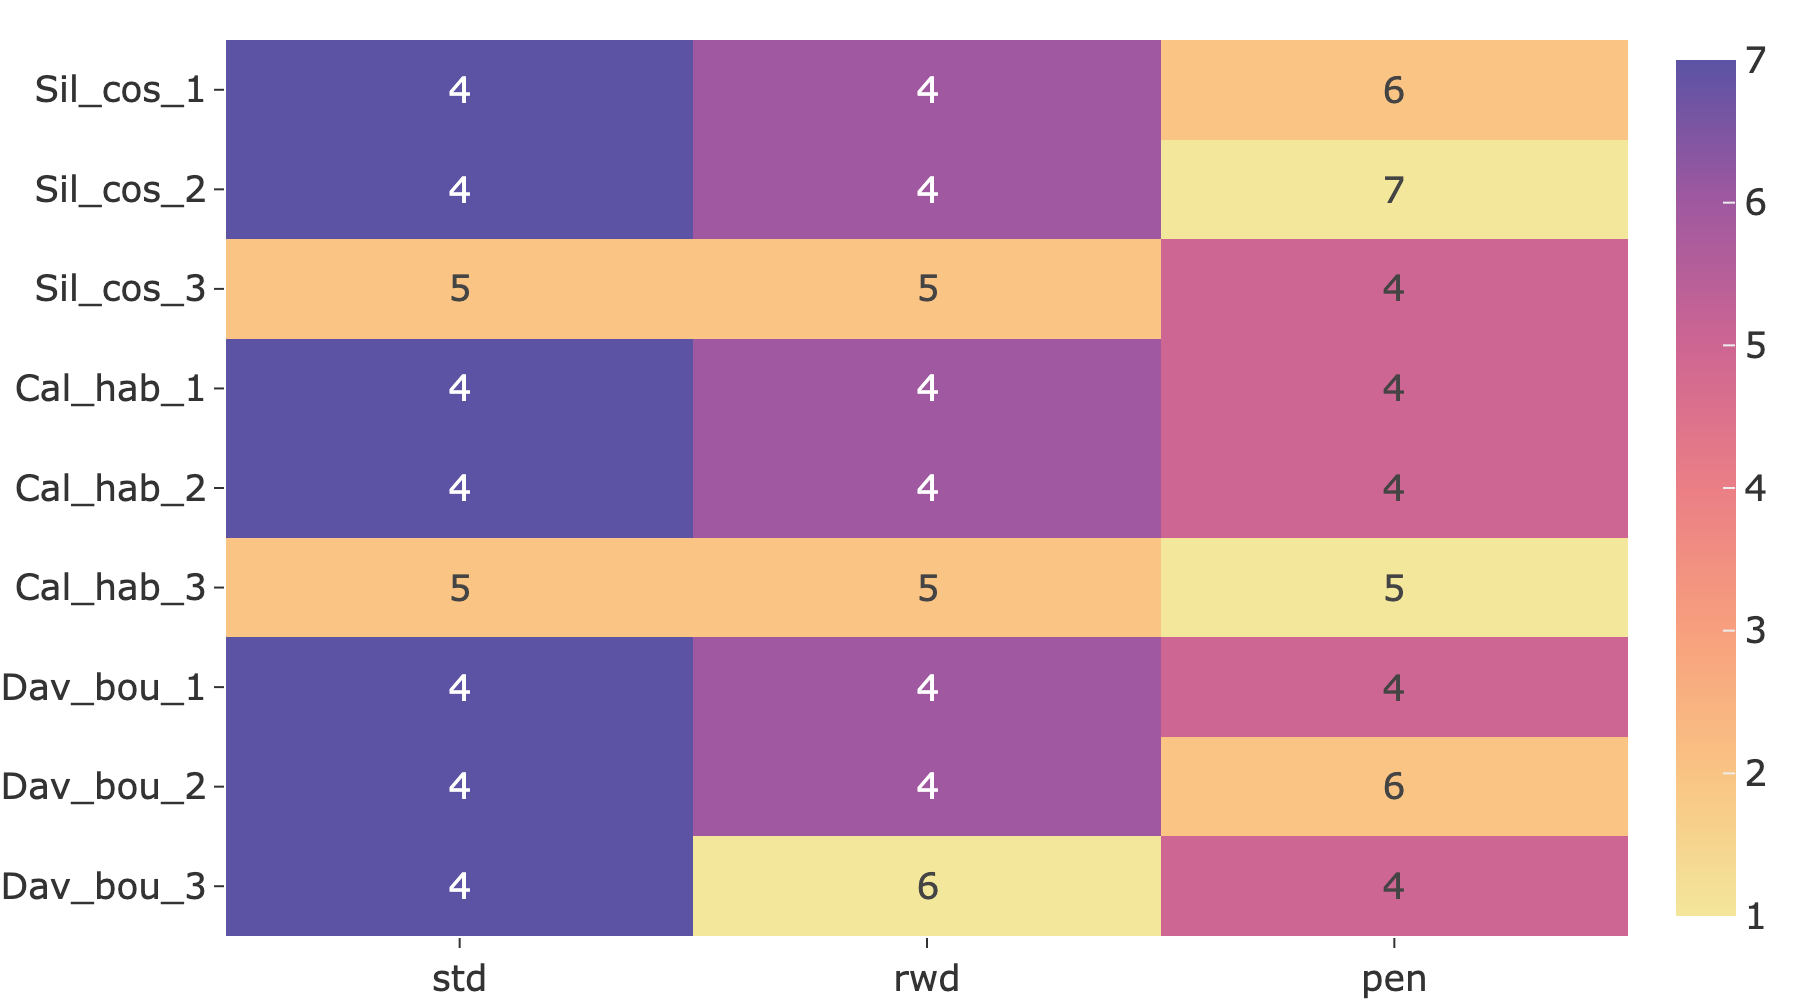
\includegraphics[width=\textwidth,keepaspectratio]{Sections/Network_I/Resources/P0/clustering/top3_cs_size_p0_tum4K_50TF_v3.png}
        \caption{Cluster size}
        \label{fig:N_I:p0_metr_size}
    \end{subfigure}
    \begin{subfigure}[!t]{1.0\textwidth}
        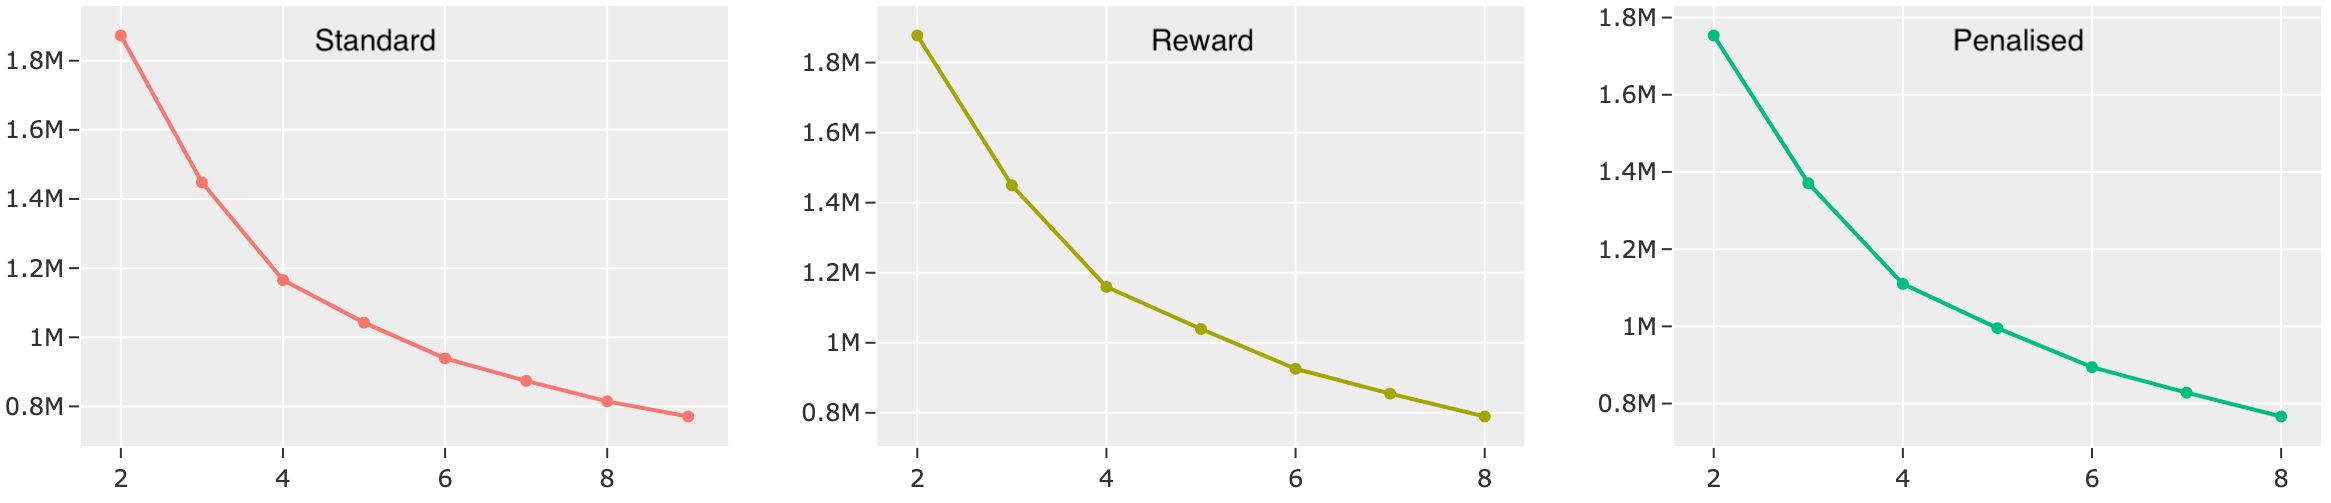
\includegraphics[width=\textwidth, keepaspectratio]{Sections/Network_I/Resources/P0/clustering/p0_elbowMethod_4K_v3.png}
        \label{fig:N_I:p0_elbow_method}
        \caption{Elbow method}
    \end{subfigure}
    \caption{Clustering models for each network type with the top three clustering scores. Colouring scale corresponds to the encounter frequency \textbf{per network type}; i.e. the count restarts for every network. A) the most likely cluster size. B) Elbow method. The two plots show that the K=4 is the common clustering configuration across all three networks by the three clustering metrics and the elbow method heurestic. }
    \label{fig:N_I:p0_top_3_metrics_II}
\end{figure}

% MIBC comparison
\subsubsection*{MIBC comparison}


To simplify the comparison, and given that the standard and reward networks are similar in performance, the MIBC subtypes comparison is performed only on the subgroups derived from the standard network. For the clustering model, K-means is used with K=4 and K=5, as the latter is the next best-performing group size across the standard and reward networks. Additionally, this number of groups aligns with the findings from the previous clustering analysis in \cref{s:cs:right_config}.

When the group size is increased to K=5, a subgroup of Basal groups (cluster 4) is identified, while the other Basal groups are further refined. The Luminal subgroups remain largely unchanged. This suggests that the Basal groups are better defined with K=5, matching previous work in the project. For these reasons, the preferred configuration is K-means with K=5 over K=4.



\begin{figure}[!htb]
    \centering
    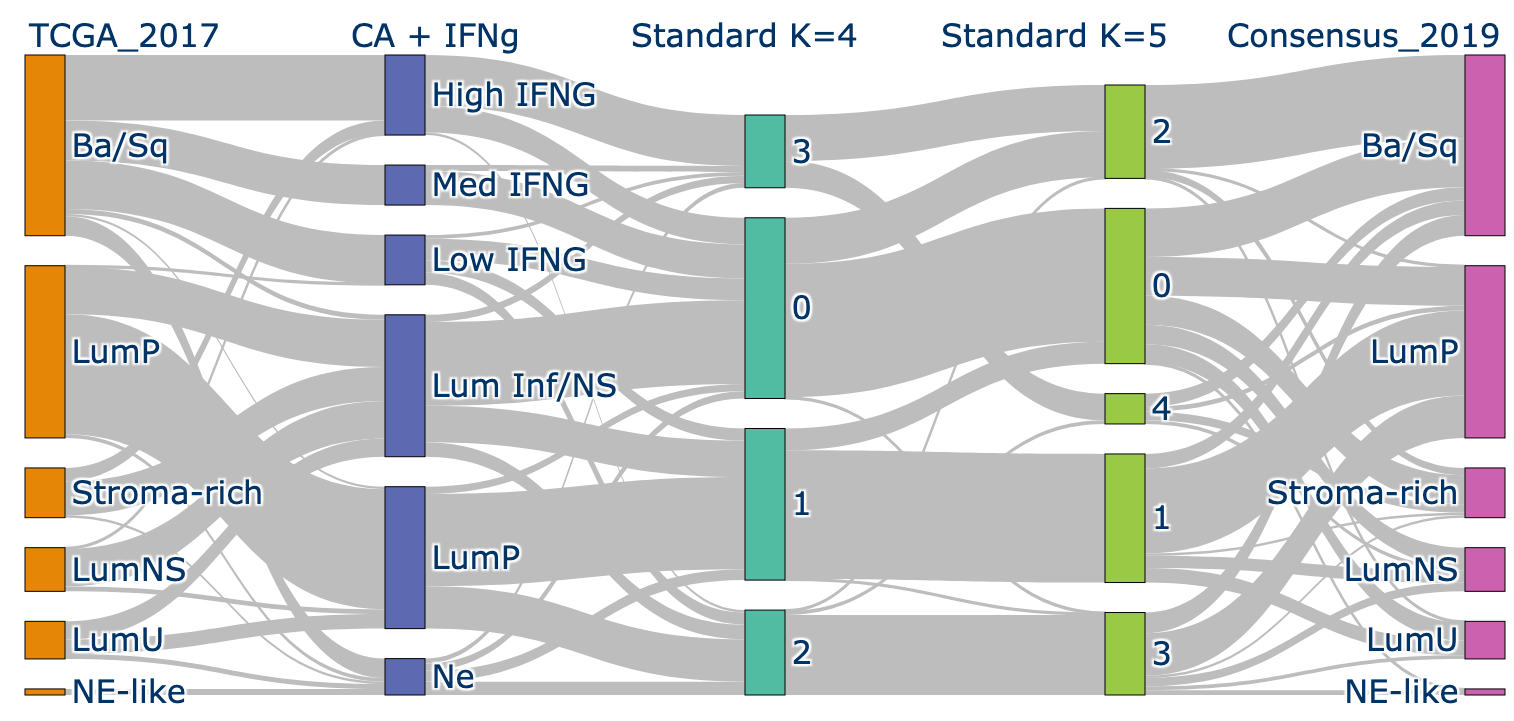
\includegraphics[width=\textwidth,keepaspectratio]{Sections/Network_I/Resources/P0/clustering/Sankey_KM_4K_v3.png}
    \caption{K-Means}
    \caption{Sankey plots for the best performing clustering model in the standard P0 network with K=4 and K=5. The derived subgroups are also compared with the previous work in the field - TCGA subtyping \citep{Robertson2017-mg} and the consensus \citet{Kamoun2020-tj} as well as the groups derived from the clustering analysis earlier in the project \cref{s:clustering_analysis}. }
    \label{fig:N_I:p0_sky_KMeans}
\end{figure}





% Align communities
\subsection{Aligning communities} \label{s:ap:align_coms}

A common challenge in unsupervised learning is the inconsistency in group labelling across different models. Typically, groups are labelled in descending order of their size. However, this approach leads to discrepancies in community labels between the standard and reward networks, complicating the analysis. To address this, community labels are synchronised by using the standard network as a reference for community numbering. Each community in the standard network is then paired with the most similar community in the reward network, based on the highest representation (i.e., the number of genes). This corresponding community in the reward network is then assigned the label from the standard network for consistency.

This method is used to align the communities in the network comparison work from \cref{s:N_I:com_analysis} for the Sankey plot between the standard and reward networks derived from the P0 dataset - see \cref{fig:N_I:p0_chg_sankey}


% gene expression across the communities
\subsection{Gene expression across communities} \label{s:ap:ge_p0_com}

The below plot, \cref{fig:ap:p0_ge_chgs}, support the work done in \cref{s:N_I:com_analysis} which analysis the genes mutations and expressions differences between the communities in the standard and reward graphs.

\begin{figure}[H]
    \centering
    \begin{subfigure}[!t]{1.0\textwidth}
    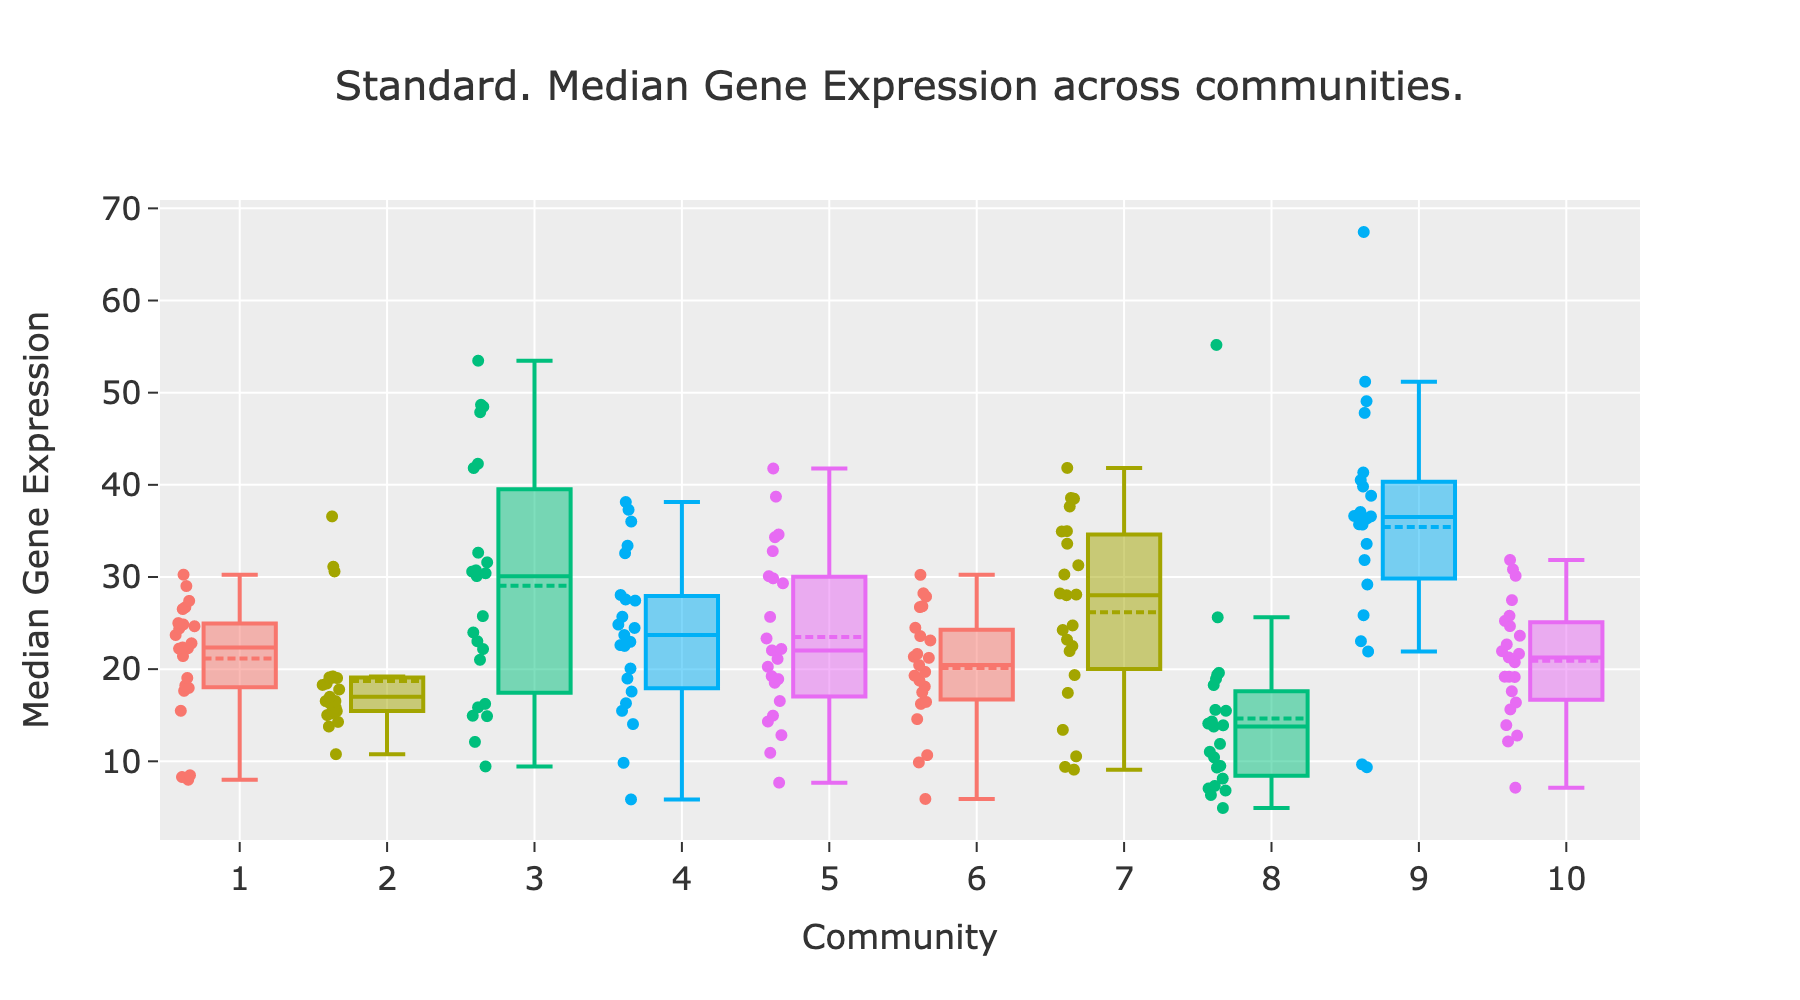
\includegraphics[width=\textwidth,keepaspectratio]{Sections/Network_I/Resources/P0/Comms/P0_standard_4K_50TF_med.png}
        \caption{Standard network}
        \label{fig:ap:p0_chg_std_exp}
    \end{subfigure}
    \begin{subfigure}[!t]{1.0\textwidth}
        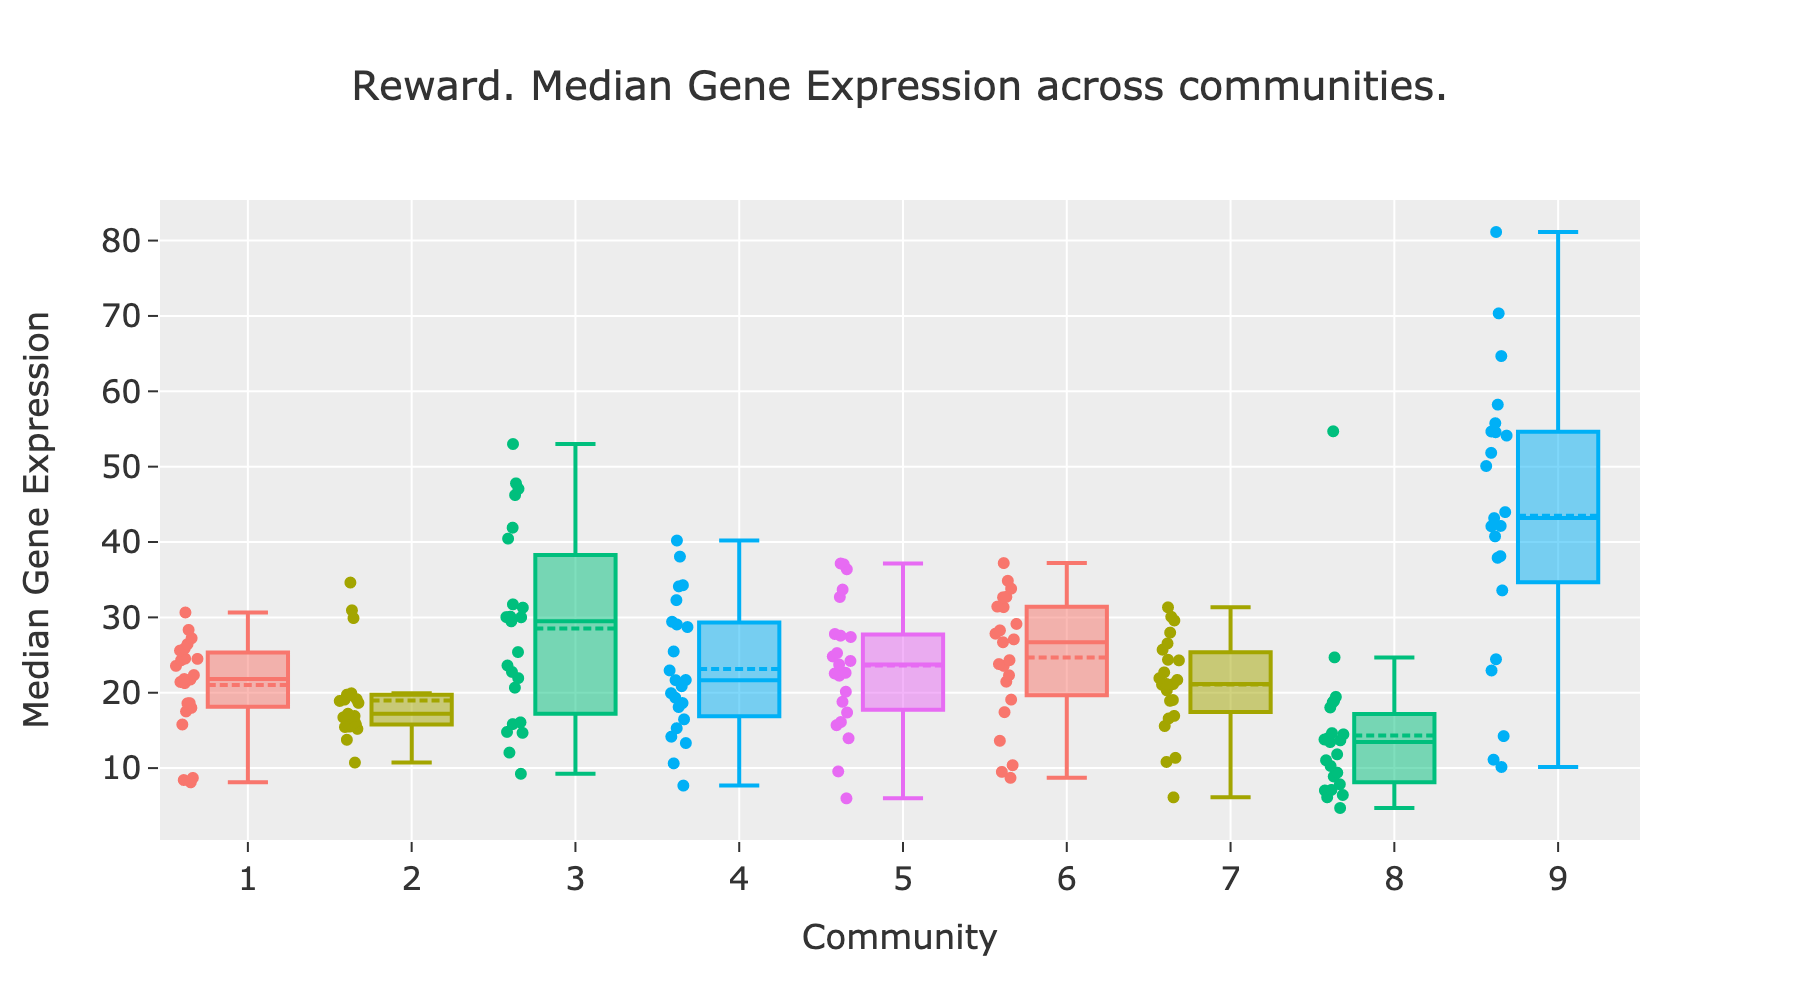
\includegraphics[width=\textwidth,keepaspectratio]{Sections/Network_I/Resources/P0/Comms/P0_norm3_4K_50TF_med.png}
            \caption{Reward network}
            \label{fig:ap:p0_chg_rwd_exp}
    \end{subfigure}
    \caption{Median gene expressions (Y-axis) across the communities (X-axis) in the standard and reward network.}
    \label{fig:ap:p0_ge_chgs}
\end{figure}

% gene rep standard
\subsection{Gene representation standard} \label{s:ap:p0_gene_rep_std}

The figure displays how many of the genes selected from the standard P0 network through ModCon (see network pipeline at \cref{fig:N_I:network_pipeline}) are found in the tumour dataset from TCGA. It shows that even when using all the expressed genes in the TCGA there are a few some genes which are not found in the tumour dataset which may have an impact on the MIBC stratification.

\begin{figure}[H]
    \centering
    \begin{subfigure}[b]{1.0\textwidth}
        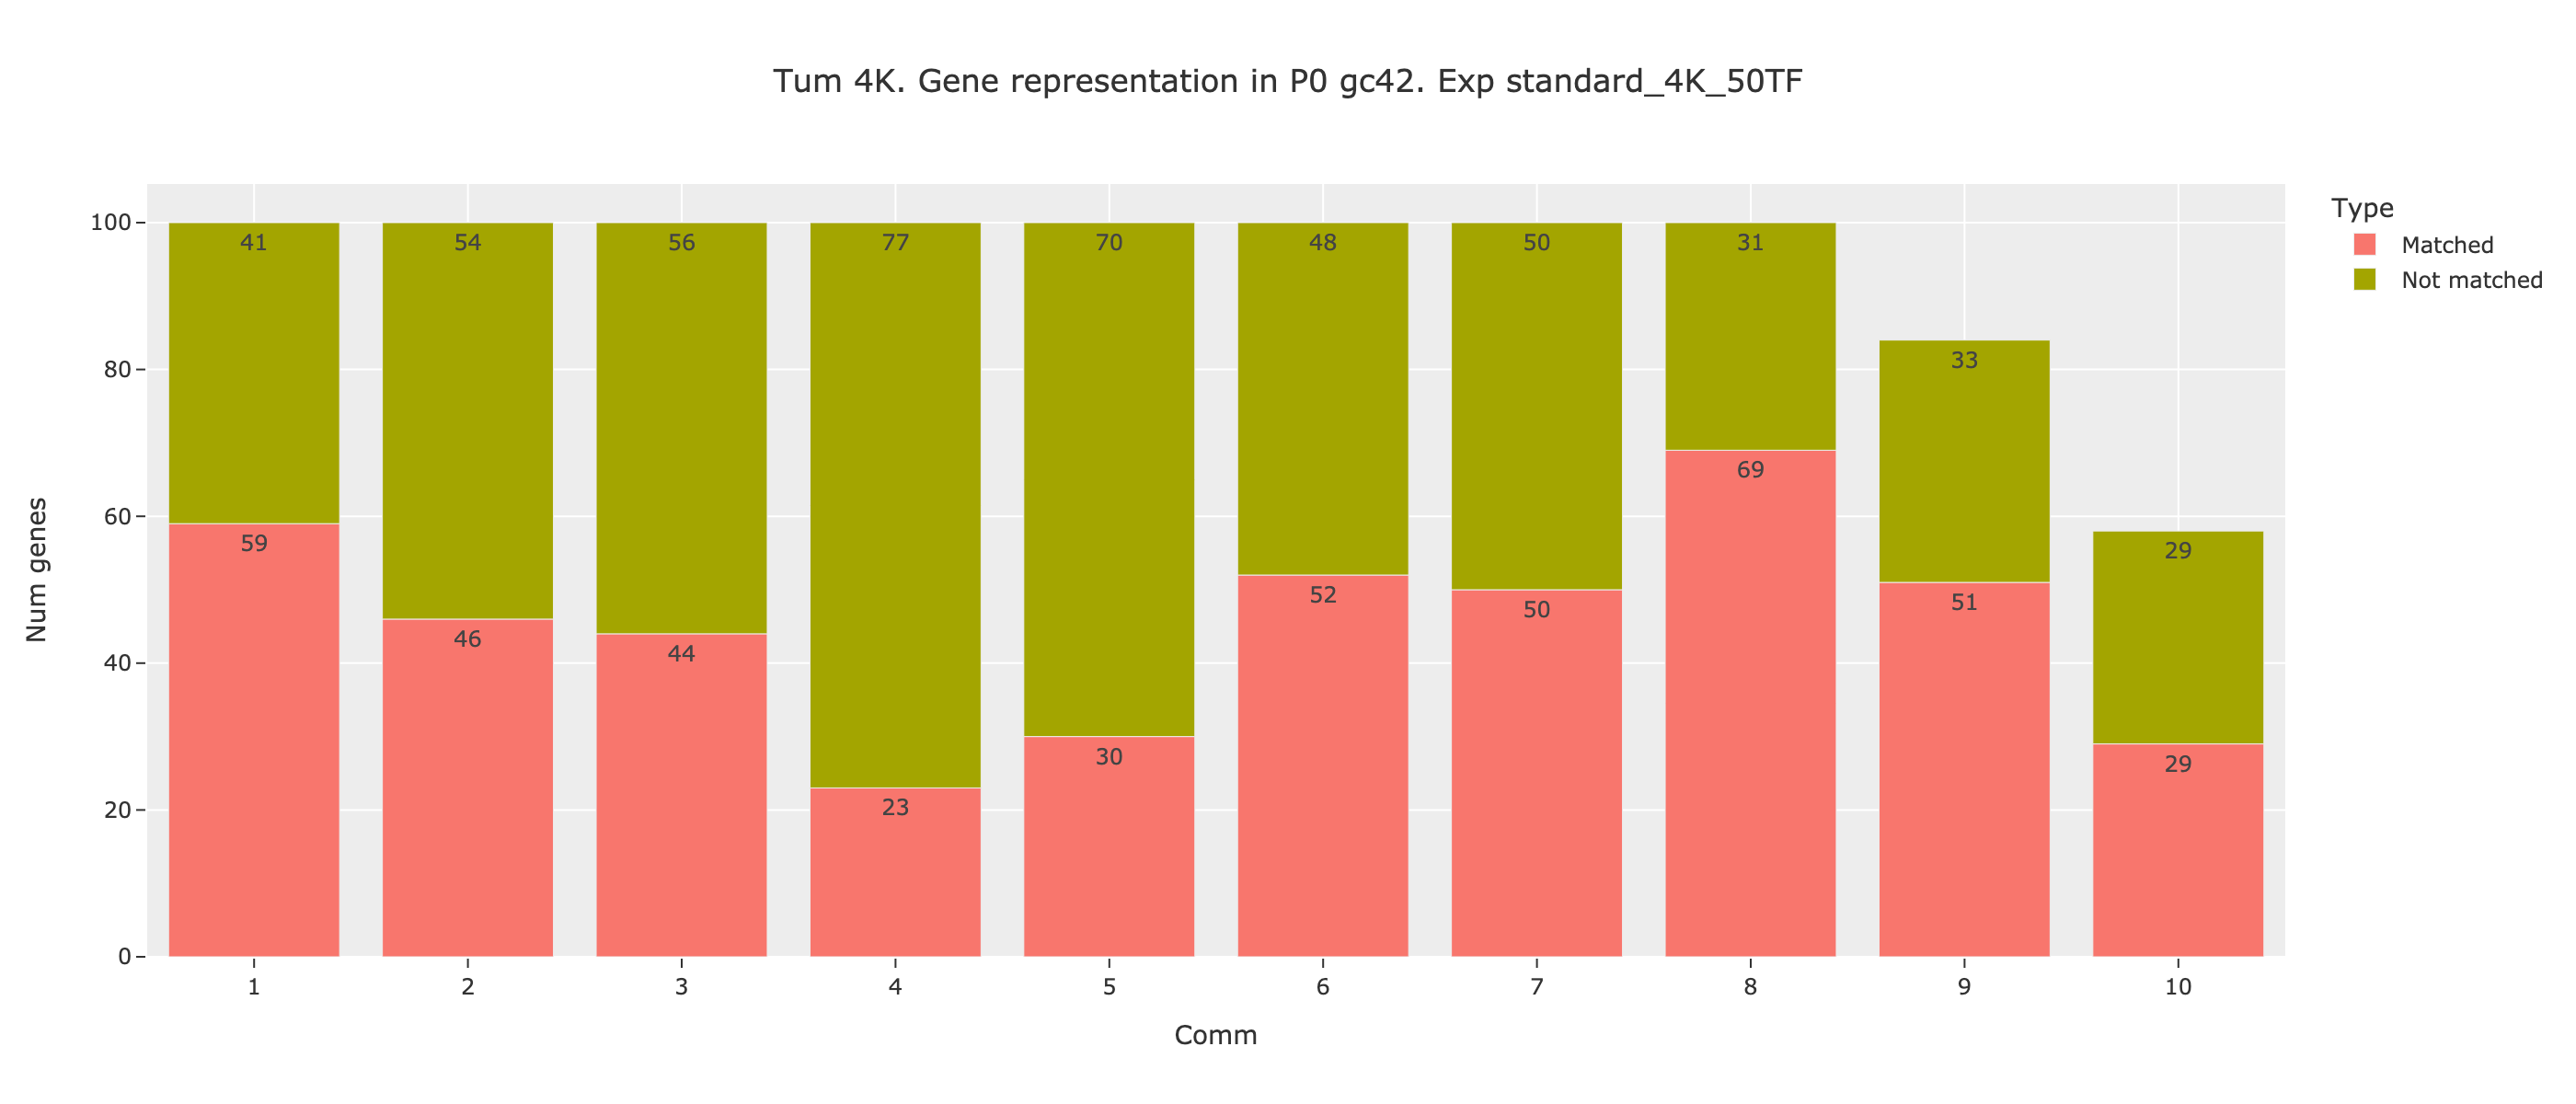
\includegraphics[width=\textwidth,keepaspectratio]{Sections/Network_I/Resources/P0/4K_p0_modConMev_rep_standard_4K_50TF_v3.png}
        \caption{The most relative varied genes}
        \label{fig:ap:std_p0_mev_sel_rep}
    \end{subfigure}
    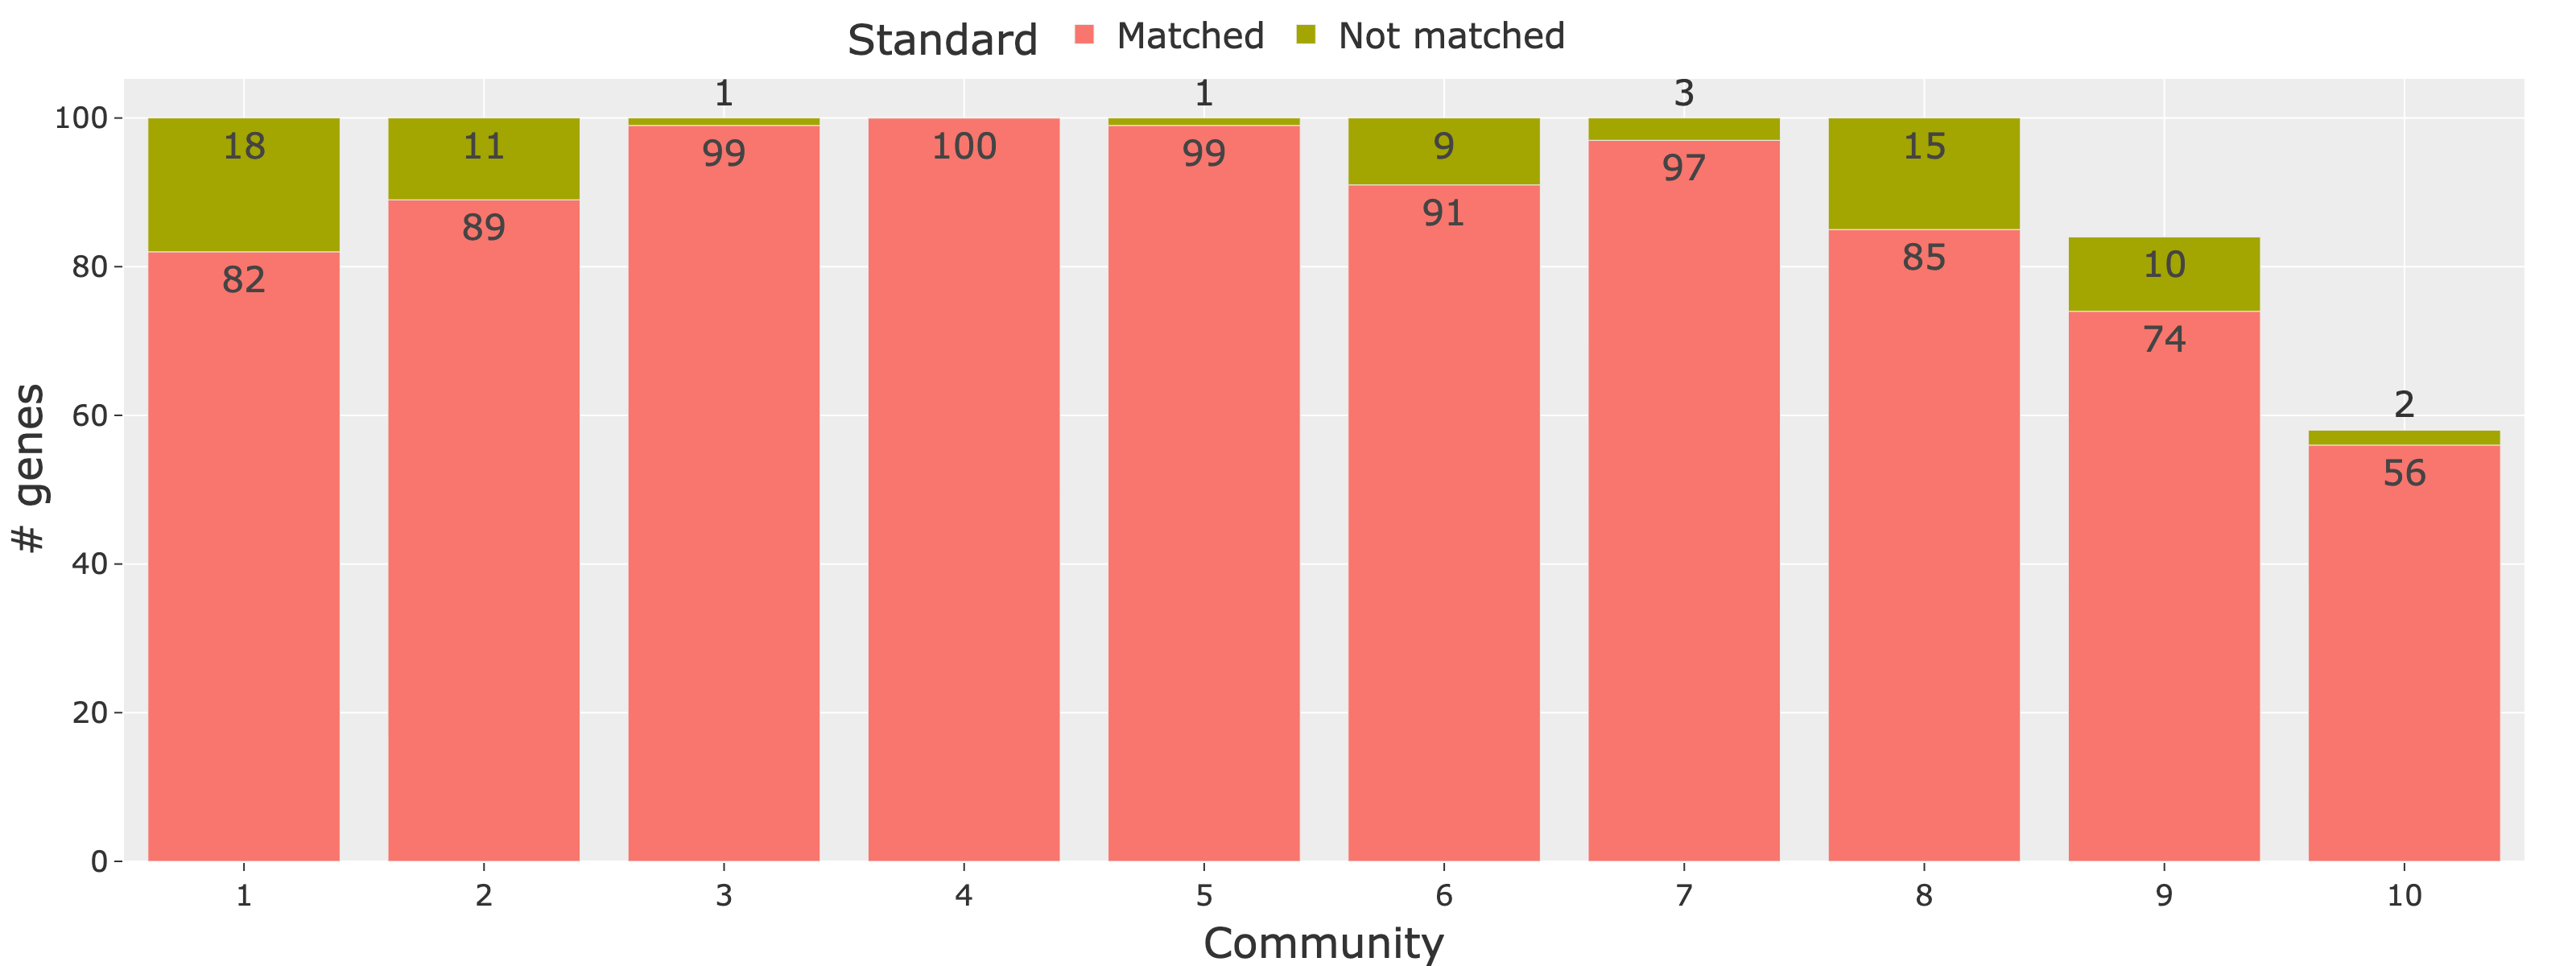
\includegraphics[width=\textwidth,keepaspectratio]{Sections/Network_I/Resources/P0/13K_p0_modConMev_rep_standard_4K_50TF_v3.png}
    \label{fig:ap:std_p0_mev_all_rep}
    \caption{Genes found in the tumour dataset for the communities across the standard network derived from the P0 samples. The two plots show that using just the top 4000 most varied genes in tumour lead to a poor representation in the genes used to compute the MEVs.}
    \label{fig:ap:std_p0_mev_rep}
\end{figure}
